\documentclass[11pt]{article}

\usepackage[T1]{fontenc}
\usepackage[utf8]{inputenc}
\usepackage{lmodern}
\usepackage[margin=0.90in]{geometry}
\usepackage{microtype}
\usepackage{amsmath,amssymb,mathtools}
\usepackage{booktabs,tabularx,multirow,array}
\usepackage{graphicx}
\usepackage{caption}
\usepackage{subcaption}
\usepackage{xcolor}
\usepackage{enumitem}
\usepackage{siunitx}
\usepackage{natbib}
\usepackage{hyperref}
\usepackage[nameinlink,capitalise,noabbrev]{cleveref}
\usepackage{tikz}
\usetikzlibrary{arrows.meta,positioning,fit,shapes.geometric}

\definecolor{Projection}{RGB}{171,85,0}
\definecolor{Invalidated}{RGB}{145,25,25}
\definecolor{ValidGreen}{RGB}{25,105,60}
\newcommand{\projected}[1]{\textcolor{Projection}{\textbf{[P:#1]}}}
\newcommand{\invalidated}[1]{\textcolor{Invalidated}{\textbf{#1}}}
\newcommand{\validmeasured}[1]{\textcolor{ValidGreen}{\textbf{#1}}}
\newcommand{\R}{\mathbb{R}}
\newcommand{\E}{\mathbb{E}}
\newcommand{\KL}{D_{\mathrm{KL}}}
\newcommand{\todofig}[1]{%
  \begin{center}
  \fbox{\begin{minipage}[c][4.2cm][c]{0.90\linewidth}
  \centering\textbf{FIGURE PLACEHOLDER}\\[4pt]
  #1
  \end{minipage}}
  \end{center}}

\hypersetup{
  colorlinks=true,
  linkcolor=black,
  citecolor=blue!50!black,
  urlcolor=blue!50!black,
  pdftitle={Reliable Goal-Conditioned Reinforcement Learning in a Vision-Only, Non-Resettable Fighting Game},
  pdfauthor={Mohamed Amine Zbida}
}

\title{\textbf{Reliable Goal-Conditioned Reinforcement Learning in a Vision-Only, Non-Resettable Fighting Game}\\[4pt]
\large Skill Transfer, Continual-Learning Measurement, and Failure-Aware Evaluation in Brawlhalla}
\author{Mohamed Amine Zbida\\\small Affiliation to be added\\\small \texttt{email to be added}}
\date{Working manuscript --- August 2026}

\begin{document}
\maketitle

\begin{center}
\fbox{\begin{minipage}{0.93\linewidth}
\small
\textbf{Draft-status convention.}
Values written as \projected{0.84} are projected placeholders inserted before the corrected experimental campaign is complete. They are intentionally searchable in the source via the macro \texttt{\textbackslash projected\{...\}} and must be replaced with measured values before publication. Normal black numbers are measurements or frozen configuration values. Historical measurements whose causal interpretation was invalidated by later integrity findings are explicitly labelled \invalidated{superseded pilot}.
\end{minipage}}
\end{center}

\begin{abstract}
Reinforcement learning in commercial real-time games differs substantially from standard simulated benchmarks: the learning system may lack privileged state, deterministic reset semantics, accelerated simulation, and parallel environment instances. We study these constraints in \emph{Brawlhalla} by constructing a vision-only reinforcement-learning agent that acquires structured competencies with goal-conditioned pretraining before transfer to a goal-independent match policy. The system combines a temporally structured visual state, an 11-dimensional masked goal representation, universal value-function approximation, residual Feature-wise Linear Modulation (FiLM), behavioral-cloning initialization, sequential transfer, PPO, replay-based preservation, policy anchoring, and gradient-conflict mitigation. The frozen goal-conditioned contract uses a 168-dimensional policy input and a discrete 27-action vocabulary; the final goal-independent policy uses a 146-dimensional observation. The perception subsystem obtains \textbf{0.984 mAP@0.5}, with AP values of \textbf{0.979}, \textbf{0.978}, and \textbf{0.995} for character, self-indicator, and weapon detection, respectively, and maximum aggregate $F_1=\textbf{0.98}$ at confidence 0.392.

A post-hoc integrity audit invalidated the causal interpretation of an initial sequential training campaign despite plausible RL logs and strong offline detector metrics. Three defects were identified: absent weapons were encoded as the valid coordinate $(0,0)$ and misread by the teacher policy; observations could alias an internal mutable environment buffer; and affected demonstration archives contained 18--64\% single-step episodes because goals were already satisfied at spawn. The historical pilot is therefore retained only as a forensic case study. Under the repaired protocol, we hypothesize final skill scores near \projected{0.84}, \projected{0.88}, \projected{0.85}, and \projected{0.58} for movement, weapon acquisition, spacing, and combat, with mean final retention around \projected{0.93} and a \projected{35\%} reduction in interactions-to-criterion from sequential transfer. The central methodological result is that high validation accuracy is insufficient to establish the correctness of a real-time RL pipeline: measurement semantics, observation ownership, task non-vacuity, and experiment provenance are part of the learning system itself.
\end{abstract}

\section{Introduction}
Deep reinforcement learning has demonstrated strong game-playing performance when interaction is mediated by simulators that provide well-defined state transitions, reset control, reproducibility, and large-scale parallelism \citep{mnih2015dqn,vinyals2019alphastar}. A commercial desktop fighting game violates most of these assumptions. The agent in this work controls a live \emph{Brawlhalla} process through keyboard-level actions while observing rendered pixels. It does not read emulator memory, does not receive privileged physical variables, cannot arbitrarily restore earlier states, and must operate under a real-time control deadline.

Let the latent game state be $s_t$, the rendered frame be $I_t$, and the action be $a_t$. The agent acts on an inferred state
\begin{equation}
\hat{s}_t = \Psi(I_{\le t}, a_{<t}),
\end{equation}
where $\Psi$ includes learned perception, identity assignment, temporal history, state normalization, validity variables, and canonicalization. Policy learning is therefore downstream of a second inference problem. A transition can be dimensionally valid while being semantically wrong; a detector can be highly accurate while the downstream state encoding is invalid; and an episode can satisfy a numerical goal without demonstrating learned behavior.

The second challenge is behavioral diversity. Fighting-game competence requires locomotion, object-directed navigation, weapon acquisition, opponent-relative spacing, recovery, and context-dependent attacks. Directly optimizing sparse match outcomes from pixels is expensive in a single live instance. We therefore treat skill learning as goal-conditioned pretraining and ask whether a shared policy can acquire structured competencies sequentially and transfer them toward unrestricted play.

This yields two research questions:
\begin{description}[leftmargin=3.8em,style=nextline]
\item[\textbf{RQ1}] Can a single vision-only goal-conditioned policy acquire and transfer heterogeneous skills efficiently?
\item[\textbf{RQ2}] What validation is required before its RL measurements are scientifically interpretable?
\end{description}

\paragraph{Contributions.}
The work makes five contributions:
\begin{enumerate}[leftmargin=1.4em]
  \item a complete vision-only real-time control pipeline for a commercial platform fighter;
  \item a masked 11-dimensional goal interface over a shared UVFA policy and critic \citep{schaul2015uvfa};
  \item residual FiLM conditioning \citep{perez2018film} and sequential behavioral/RL transfer across movement, weapon acquisition, spacing, and combat;
  \item an explicit retention/amnesia protocol that reevaluates previous skills after each curriculum phase;
  \item a failure-aware methodology motivated by three concrete defects that standard detector and dataset validation did not expose.
\end{enumerate}

\section{Related Work}
\subsection{Goal-conditioned value functions}
Universal Value Function Approximators extend conventional value functions to explicit goals \citep{schaul2015uvfa}:
\begin{equation}
V^{\pi}(s,g) = \E_{\pi}\!\left[\sum_{k=0}^{\infty}\gamma^k r_{t+k}\mid s_t=s, g_t=g\right].
\end{equation}
A corresponding policy is $\pi_\theta(a\mid s,g)$. The formulation permits one parameterized policy to share representations across related objectives.

\subsection{Conditioning through FiLM}
FiLM generates feature-wise affine transformations from conditioning information \citep{perez2018film}:
\begin{equation}
\operatorname{FiLM}(h;\gamma,\beta)=\gamma\odot h+\beta.
\end{equation}
Our network uses a residual form so goal conditioning can alter intermediate state features without deleting an unconditioned pathway.

\subsection{Behavioral initialization and relabeling}
Behavioral cloning supplies an action prior before expensive online interaction, while hindsight-style relabeling can improve reuse of trajectories in goal-conditioned settings \citep{andrychowicz2017her}. In this project, the demonstrations initialize the first competency and later phases receive additional goal-relabelled behavioral updates before PPO.

\subsection{Continual learning and conflicting gradients}
Sequential training risks catastrophic forgetting \citep{kirkpatrick2017ewc}. We measure retention explicitly and combine replay, policy anchoring, and a PCGrad-style projection when preservation and current-skill gradients conflict \citep{yu2020pcgrad}.

\section{Problem Formulation}
We model the live interaction as a partially observable controlled process
\begin{equation}
\mathcal{P}=(\mathcal{S},\mathcal{A},\mathcal{O},T,\Omega,R,\gamma).
\end{equation}
The agent does not observe $s_t\in\mathcal S$ directly. Instead it receives image observations $I_t\in\mathcal O$ and constructs an approximate state with explicit short-term history:
\begin{equation}
\hat{s}_t=\Psi(I_t,I_{t-2},I_{t-4},I_{t-8},a_{t-1},a_{t-3},a_{t-5},a_{t-9}).
\end{equation}
The frozen goal-conditioned contract has
\begin{equation}
\dim(o_t)=168,\qquad \dim(g_t)=11,\qquad |\mathcal A|=27.
\end{equation}
The final unrestricted match policy uses a 146-dimensional observation and the same 27-action vocabulary. The distinction is intentional: skill pretraining is goal-conditioned, whereas the final match policy is goal-independent.

\section{System Architecture}
\begin{figure}[t]
\centering
\resizebox{0.98\linewidth}{!}{%
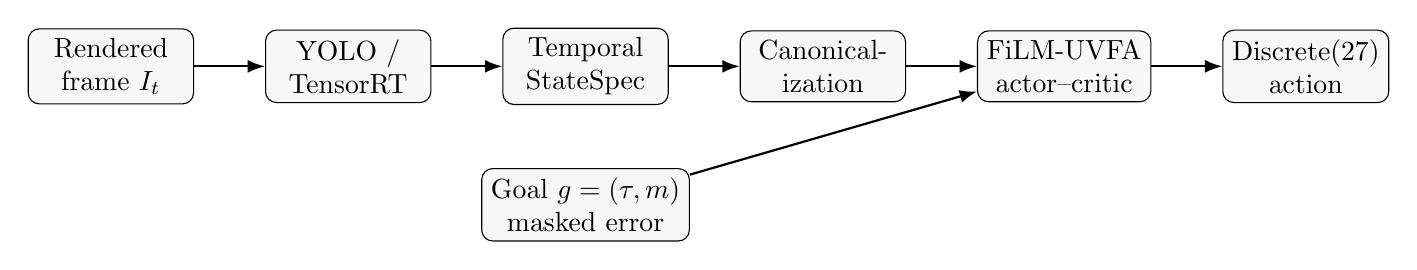
\begin{tikzpicture}[
  node distance=8mm and 9mm,
  box/.style={draw, rounded corners, align=center, minimum height=9mm, minimum width=21mm, fill=black!3},
  arr/.style={-{Latex[length=2.2mm]}, thick}
]
\node[box] (frame) {Rendered\\frame $I_t$};
\node[box,right=of frame] (det) {YOLO /\\TensorRT};
\node[box,right=of det] (state) {Temporal\\StateSpec};
\node[box,right=of state] (canon) {Canonical-\\ization};
\node[box,below=of state] (goal) {Goal $g=(\tau,m)$\\masked error};
\node[box,right=of canon] (film) {FiLM-UVFA\\actor--critic};
\node[box,right=of film] (act) {Discrete(27)\\action};
\draw[arr] (frame) -- (det);
\draw[arr] (det) -- (state);
\draw[arr] (state) -- (canon);
\draw[arr] (canon) -- (film);
\draw[arr] (goal) -- (film);
\draw[arr] (film) -- (act);
\end{tikzpicture}%
}
\caption{High-level control path. Goal-conditioned pretraining supplies a goal vector to the shared actor--critic; the final match policy removes that explicit goal channel while retaining the learned representation.}
\label{fig:system}
\end{figure}

\subsection{Perception}
The object detector predicts three principal classes:
\begin{equation}
\mathcal C=\{\text{character},\text{indicator\_self},\text{weapon}\}.
\end{equation}
The self-indicator resolves the controlled fighter among visually similar character detections. A detector prediction is represented as
\begin{equation}
b_i=(x_i,y_i,w_i,h_i,c_i,p_i),
\end{equation}
with class $c_i$ and confidence $p_i$. Derived normalized features include self/opponent positions, relative geometry, weapon location when valid, and other context variables.

An auxiliary weapon-state classifier estimates whether fighters are armed. The frozen configuration records cross-validation accuracy 0.957 and a runtime minimum confidence of 0.7.

\subsection{Temporal history}
A single frame does not reveal velocity, recently initiated attacks, or recovery direction. Selected variables are therefore stacked at offsets
\begin{equation}
H_t(z)=[z_t,z_{t-2},z_{t-4},z_{t-8}],
\end{equation}
with previous-action semantics supplied at corresponding recent offsets. This is a deliberate alternative to making the entire policy recurrent.

\subsection{Canonicalization}
Horizontal symmetry is exploited by mapping observations to a canonical orientation. If the opponent lies on the noncanonical side, horizontal coordinates are reflected, e.g.
\begin{equation}
x' = 1-x,
\end{equation}
and directional actions are swapped. This reduces duplicated learning of left/right-equivalent behavior.

\section{Goal Representation and Reward}
Each skill uses
\begin{equation}
g=(\tau,m),\qquad \tau\in[0,1]^{11},\quad m\in\{0,1\}^{11},
\end{equation}
where $\tau$ is the target vector and $m$ selects active coordinates. Let $\phi(\hat{s}_t)$ extract goal-relevant state variables. The signed masked error is
\begin{equation}
e_t=m\odot(\phi(\hat{s}_t)-\tau).
\end{equation}
To prevent goals with more active dimensions from receiving mechanically larger errors, the scalar error is normalized by active mask mass:
\begin{equation}
E_t=\frac{\sum_i m_i|e_{t,i}|}{\sum_i m_i+\epsilon}.
\end{equation}
Progress is
\begin{equation}
\Delta E_t=E_{t-1}-E_t,
\end{equation}
and the dense reward component is
\begin{equation}
r_t^{\mathrm{goal}}=\alpha\Delta E_t.
\end{equation}
The complete phase-specific reward adds semantically meaningful events:
\begin{equation}
r_t=\operatorname{clip}\!\left(\alpha\Delta E_t+r_t^{\mathrm{event}}+r_t^{\mathrm{terminal}},-r_{\max},r_{\max}\right).
\end{equation}

The curriculum contains movement, weapon acquisition, spacing, combat, and recovery families. The initial live pilot activated the first four and deferred recovery/all-skill consolidation.

\section{Residual FiLM Universal Policy}
The state pathway receives a feature vector containing the reconstructed observation, masked goal error, goal mask, and motion-alignment terms:
\begin{equation}
z_s=[\hat{s}_t,e_t,m,q_t],\qquad h_s=f_s(z_s).
\end{equation}
The goal pathway computes
\begin{equation}
z_g=[\tau,m],\qquad h_g=f_g(z_g).
\end{equation}
Goal features generate modulation parameters
\begin{equation}
[\gamma_g,\beta_g]=f_{\mathrm{FiLM}}(h_g),
\end{equation}
and the residual modulation is
\begin{equation}
\tilde h_s=h_s+\gamma_g\odot h_s+\beta_g.
\end{equation}
Actor and critic heads estimate
\begin{equation}
\pi_\theta(a\mid \hat{s},g),\qquad V_\theta(\hat{s},g).
\end{equation}
This lets the same physical observation be represented differently under, for example, movement and combat goals.

\section{Behavioral Pretraining and Sequential Transfer}
The frozen demonstration manifest contains 7,938 samples across 200 episodes. \Cref{tab:demos} summarizes the four active skill archives.

\begin{table}[t]
\centering
\caption{Frozen demonstration archive. These counts describe the pre-repair data contract; later integrity findings require repaired archives for final claims.}
\label{tab:demos}
\begin{tabular}{lrrrr}
\toprule
Skill & Samples & Episodes & Action entropy & Attack rate\\
\midrule
Movement & 1,596 & 50 & 0.715 & 0.000\\
Weapon acquisition & 3,366 & 50 & 0.671 & 0.000\\
Spacing & 1,230 & 50 & 0.732 & 0.000\\
Combat & 1,746 & 50 & 0.844 & 0.359\\
\midrule
Total & 7,938 & 200 & -- & --\\
\bottomrule
\end{tabular}
\end{table}

Behavioral cloning minimizes
\begin{equation}
\mathcal L_{\mathrm{BC}}=-\E_{(s,g,a)\sim D}\log\pi_\theta(a\mid s,g).
\end{equation}
The frozen configuration uses eight BC epochs for later phases, batch size 512, learning rate $2\times10^{-4}$, entropy coefficient 0.001, and goal relabeling. Sequential initialization follows
\begin{equation}
\theta_W^{(0)}\leftarrow\theta_M^*,\quad
\theta_S^{(0)}\leftarrow\theta_W^*,\quad
\theta_C^{(0)}\leftarrow\theta_S^*.
\end{equation}

\section{PPO and Continual-Learning Stabilization}
The PPO clipped objective is \citep{schulman2017ppo}
\begin{equation}
L^{\mathrm{CLIP}}(\theta)=\E_t\left[\min\left(r_t(\theta)\hat A_t,\operatorname{clip}(r_t(\theta),1-\epsilon,1+\epsilon)\hat A_t\right)\right],
\end{equation}
with
\begin{equation}
r_t(\theta)=\frac{\pi_\theta(a_t\mid s_t,g_t)}{\pi_{\theta_{\mathrm{old}}}(a_t\mid s_t,g_t)}.
\end{equation}
The core loss combines policy, value, and entropy terms. Preservation adds historical replay and a frozen-policy anchor:
\begin{equation}
\mathcal L_{\mathrm{anchor}}=\KL\!\left(\pi_{\mathrm{ref}}(\cdot\mid s,g)\,\|\,\pi_\theta(\cdot\mid s,g)\right),
\end{equation}
\begin{equation}
\mathcal L_{\mathrm{aux}}=\lambda_{\mathrm{KL}}\mathcal L_{\mathrm{anchor}}+\lambda_{\mathrm{BC}}\mathcal L_{\mathrm{BC}}.
\end{equation}
When current-skill gradient $g_c$ conflicts with preservation gradient $g_p$,
\begin{equation}
g_c^\top g_p<0,
\end{equation}
a PCGrad-style projection removes the conflicting component:
\begin{equation}
g_c' = g_c-\frac{g_c^\top g_p}{\|g_p\|_2^2+\epsilon}g_p.
\end{equation}

\section{Retention and Amnesia}
For skill $i$ evaluated after sequential stage $j$, let the normalized competency score be $S_{i,j}\in[0,1]$. The best previous score is
\begin{equation}
S_i^{\max}(j)=\max_{k\le j}S_{i,k}.
\end{equation}
Retention and amnesia are
\begin{equation}
R_{i,j}=\frac{S_{i,j}}{S_i^{\max}(j)+\epsilon},
\end{equation}
\begin{equation}
A_{i,j}=\max(0,1-R_{i,j}).
\end{equation}
The project uses a preservation gate
\begin{equation}
R_{i,j}\ge0.85.
\end{equation}
A curriculum checkpoint is therefore not judged only by the newly trained diagonal score; all previously learned competencies are reevaluated.

\section{Experimental Integrity as Part of the Method}
The initial pilot exposed a central issue: optimization is only meaningful if the data preserve the semantics assumed by the objective. Three defects are treated as methodological findings rather than hidden implementation details.

\subsection{Typed missingness}
An absent weapon was originally represented as $(0,0)$. Downstream teacher logic interpreted this sentinel as a legitimate point. If weapon validity is $v_t\in\{0,1\}$ and position is $p_t\in\R^2$, the corrected observation is
\begin{equation}
w_t=(v_t,p_t),
\end{equation}
and weapon-dependent control must satisfy
\begin{equation}
a_t^{\mathrm{pickup}}=\mathbf 1[v_t=1]\,f(p_{\mathrm{self}},p_t,\ldots).
\end{equation}
The post-hoc teacher audit found that approximately 82.6\% of pickup presses occurred while no weapon was on the ground, with pickup pressed roughly 14\% of the time overall. The original weapon behavioral prior was therefore not evidence of a correctly acquired pickup skill.

\subsection{Observation ownership}
The environment previously returned an internal mutable observation buffer instead of an independent value. If a stored reference $o_t$ aliases buffer $B$ and the next step mutates $B$, then a transition intended to be
\begin{equation}
(o_t,a_t,r_t,o_{t+1})
\end{equation}
can degenerate toward
\begin{equation}
(o_{t+1},a_t,r_t,o_{t+1}).
\end{equation}
The corrected invariant is that consecutive mutable observations do not share writable memory.

\subsection{Non-vacuous competency episodes}
Affected demonstration archives contained 18--64\% single-step episodes because sampled goals were already satisfied at spawn. A valid competency episode now requires initial violation
\begin{equation}
E_0>\epsilon_{\mathrm{init}}
\end{equation}
and subsequent achievement
\begin{equation}
\exists t>0:E_t<\epsilon_{\mathrm{success}}.
\end{equation}
For skills where simple threshold crossing is insufficient, the episode can additionally require minimum progress
\begin{equation}
E_0-\min_t E_t>\delta.
\end{equation}

\subsection{Why ordinary validation did not catch the defects}
The frozen manifest marked all four demonstration archives as PASS, and detector performance was very high. Yet none of those checks verified missing-object semantics, temporal ownership, or whether a ``successful'' episode required action. We therefore treat the following invariants as part of the experimental method:
\begin{enumerate}[leftmargin=1.4em]
  \item \textbf{Observation ownership:} mutable observations may not alias across steps.
  \item \textbf{Missingness consistency:} invalid values cannot drive geometry-based decisions.
  \item \textbf{Reward cross-check:} sampled logged rewards are recomputed from transition data.
  \item \textbf{Non-vacuity:} competence evaluation begins outside the success set.
  \item \textbf{Action plausibility:} state-dependent teacher actions obey explicit invariants.
  \item \textbf{Train/serve equivalence:} recorded frames produce numerically equivalent features under training and runtime extraction.
\end{enumerate}

\section{Experiment Provenance and Data Status}
A reproducible experiment is identified by more than a commit hash. We use the conceptual identity
\begin{equation}
\mathcal E=(H_{\mathrm{source}},H_{\mathrm{config}},H_{\mathrm{data}},H_{\mathrm{checkpoint}},\mathrm{seed}).
\end{equation}
The frozen manifest records commit \texttt{6b05852c8b62ac1853f64dc923fe6f481be5bdbc} but also records a dirty worktree and explicitly warns that the commit alone does not identify the exact source state. Future live runs should therefore use a clean source checkpoint or an additional content hash.

The supplied world-replay archive contains three relevant collections: 18 root exploratory sessions with 69,192 transitions; four dedicated three-hour skill sessions with 361,472 transitions; and one repair session with 4,096 transitions. Sessions before 2026-08-12 23:00 are considered affected by the observation-aliasing defect. The historical three-hour skill campaign is retained but superseded because it also depends on invalid teacher/demo semantics.

\begin{table}[t]
\centering
\caption{Evidence taxonomy used in this manuscript.}
\label{tab:provenance}
\begin{tabularx}{\linewidth}{lrrX}
\toprule
Artifact family & Sessions & Transitions & Scientific status\\
\midrule
Exploratory world replay & 18 & 69,192 & Mixed provenance; pre-2026-08-12 23:00 sessions invalidated by observation aliasing\\
Dedicated 3h replay & 4 & 361,472 & Historical/superseded for final method claims\\
Repair replay & 1 & 4,096 & Post-repair diagnostic collection\\
Detector validation & -- & -- & Valid for perception metrics\\
Corrected sequential chain & \projected{4 phases} & \projected{TBD} & Required for headline RL claims\\
\bottomrule
\end{tabularx}
\end{table}

\section{Experimental Protocol}
The frozen game configuration uses Wu Shang against one Easy Mordex opponent on Small Brawlhaven at $1920\times1080$ resolution. The skill pilot is goal-conditioned; the final agent is goal-independent. PPO uses rollout length 512, batch size 256, seed 42, and CPU execution in the frozen pilot configuration.

The original sequential gate used only two evaluation episodes per skill. That is suitable for software smoke testing but not for a research estimate. The corrected campaign should use at least \projected{30} deterministic evaluation episodes per skill/checkpoint where practical, reporting confidence intervals over evaluation episodes and clearly separating evaluation uncertainty from training-seed uncertainty.

\paragraph{Primary corrected sequence.}
\begin{equation}
\text{Movement}\rightarrow\text{Weapon}\rightarrow\text{Spacing}\rightarrow\text{Combat}.
\end{equation}
For each phase, the final paper should retain episode/step logs, the exact model checkpoint, evaluation output for all skills learned so far, and integrity-test summaries.

\section{Results I: Perception and Runtime}
\subsection{Detector validation}
The supplied validation curves show class AP@0.5 values of 0.979 for character, 0.978 for the self-indicator, and 0.995 for weapon, with aggregate
\begin{equation}
\mathrm{mAP@0.5}=\mathbf{0.984}.
\end{equation}
The maximum aggregate F1 is
\begin{equation}
F_1^*=\mathbf{0.98}
\end{equation}
at confidence 0.392.

\begin{figure}[t]
\centering
\begin{subfigure}{0.49\linewidth}
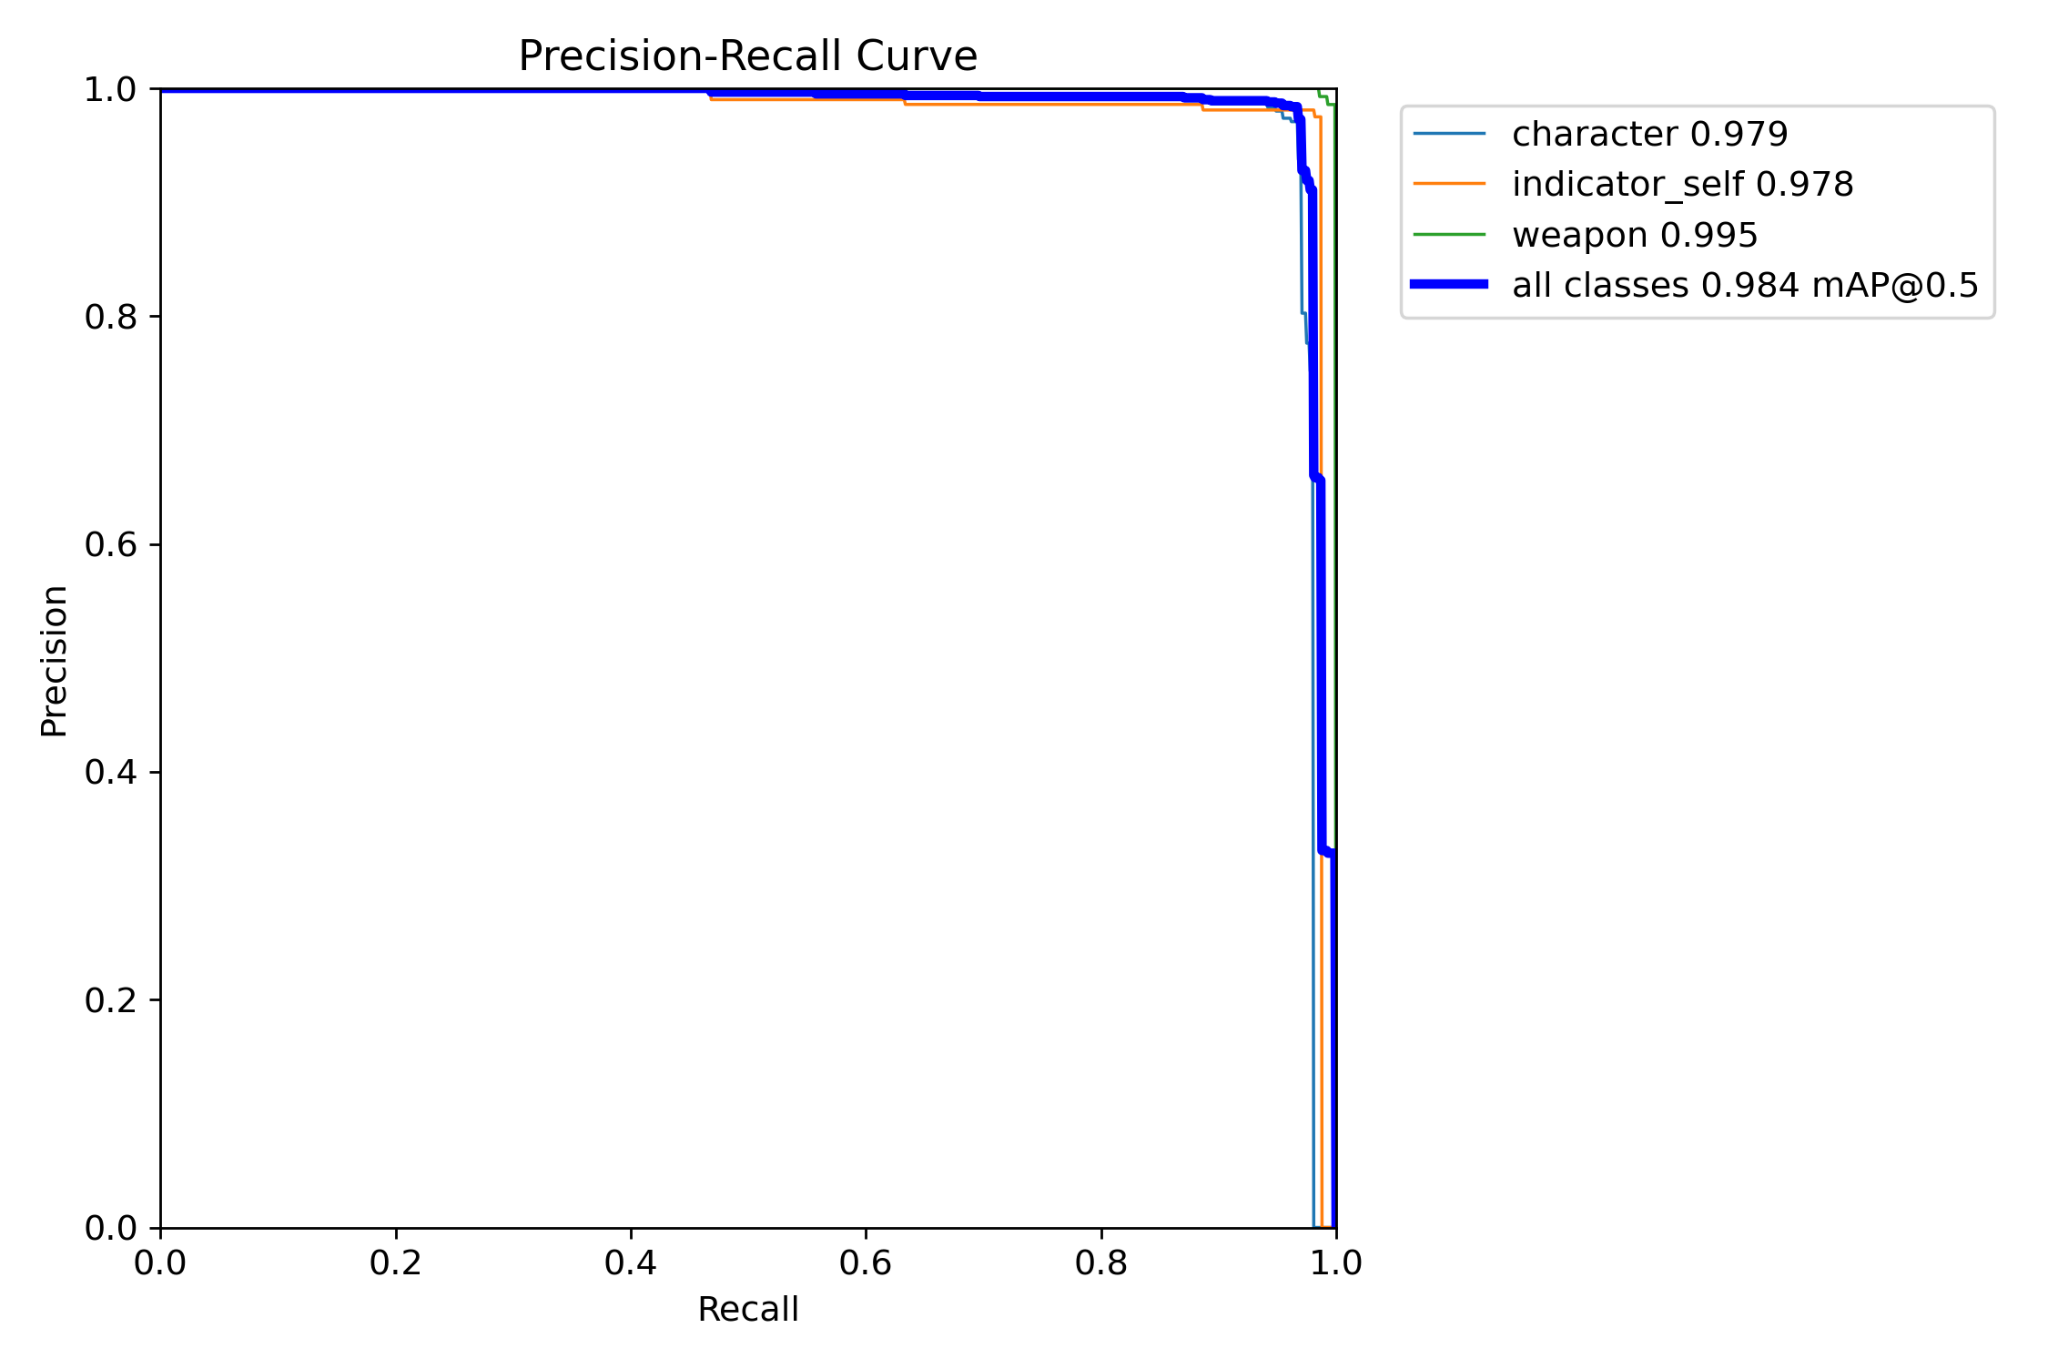
\includegraphics[width=\linewidth]{figures/detector_pr.png}
\caption{Precision--recall curve.}
\end{subfigure}\hfill
\begin{subfigure}{0.49\linewidth}
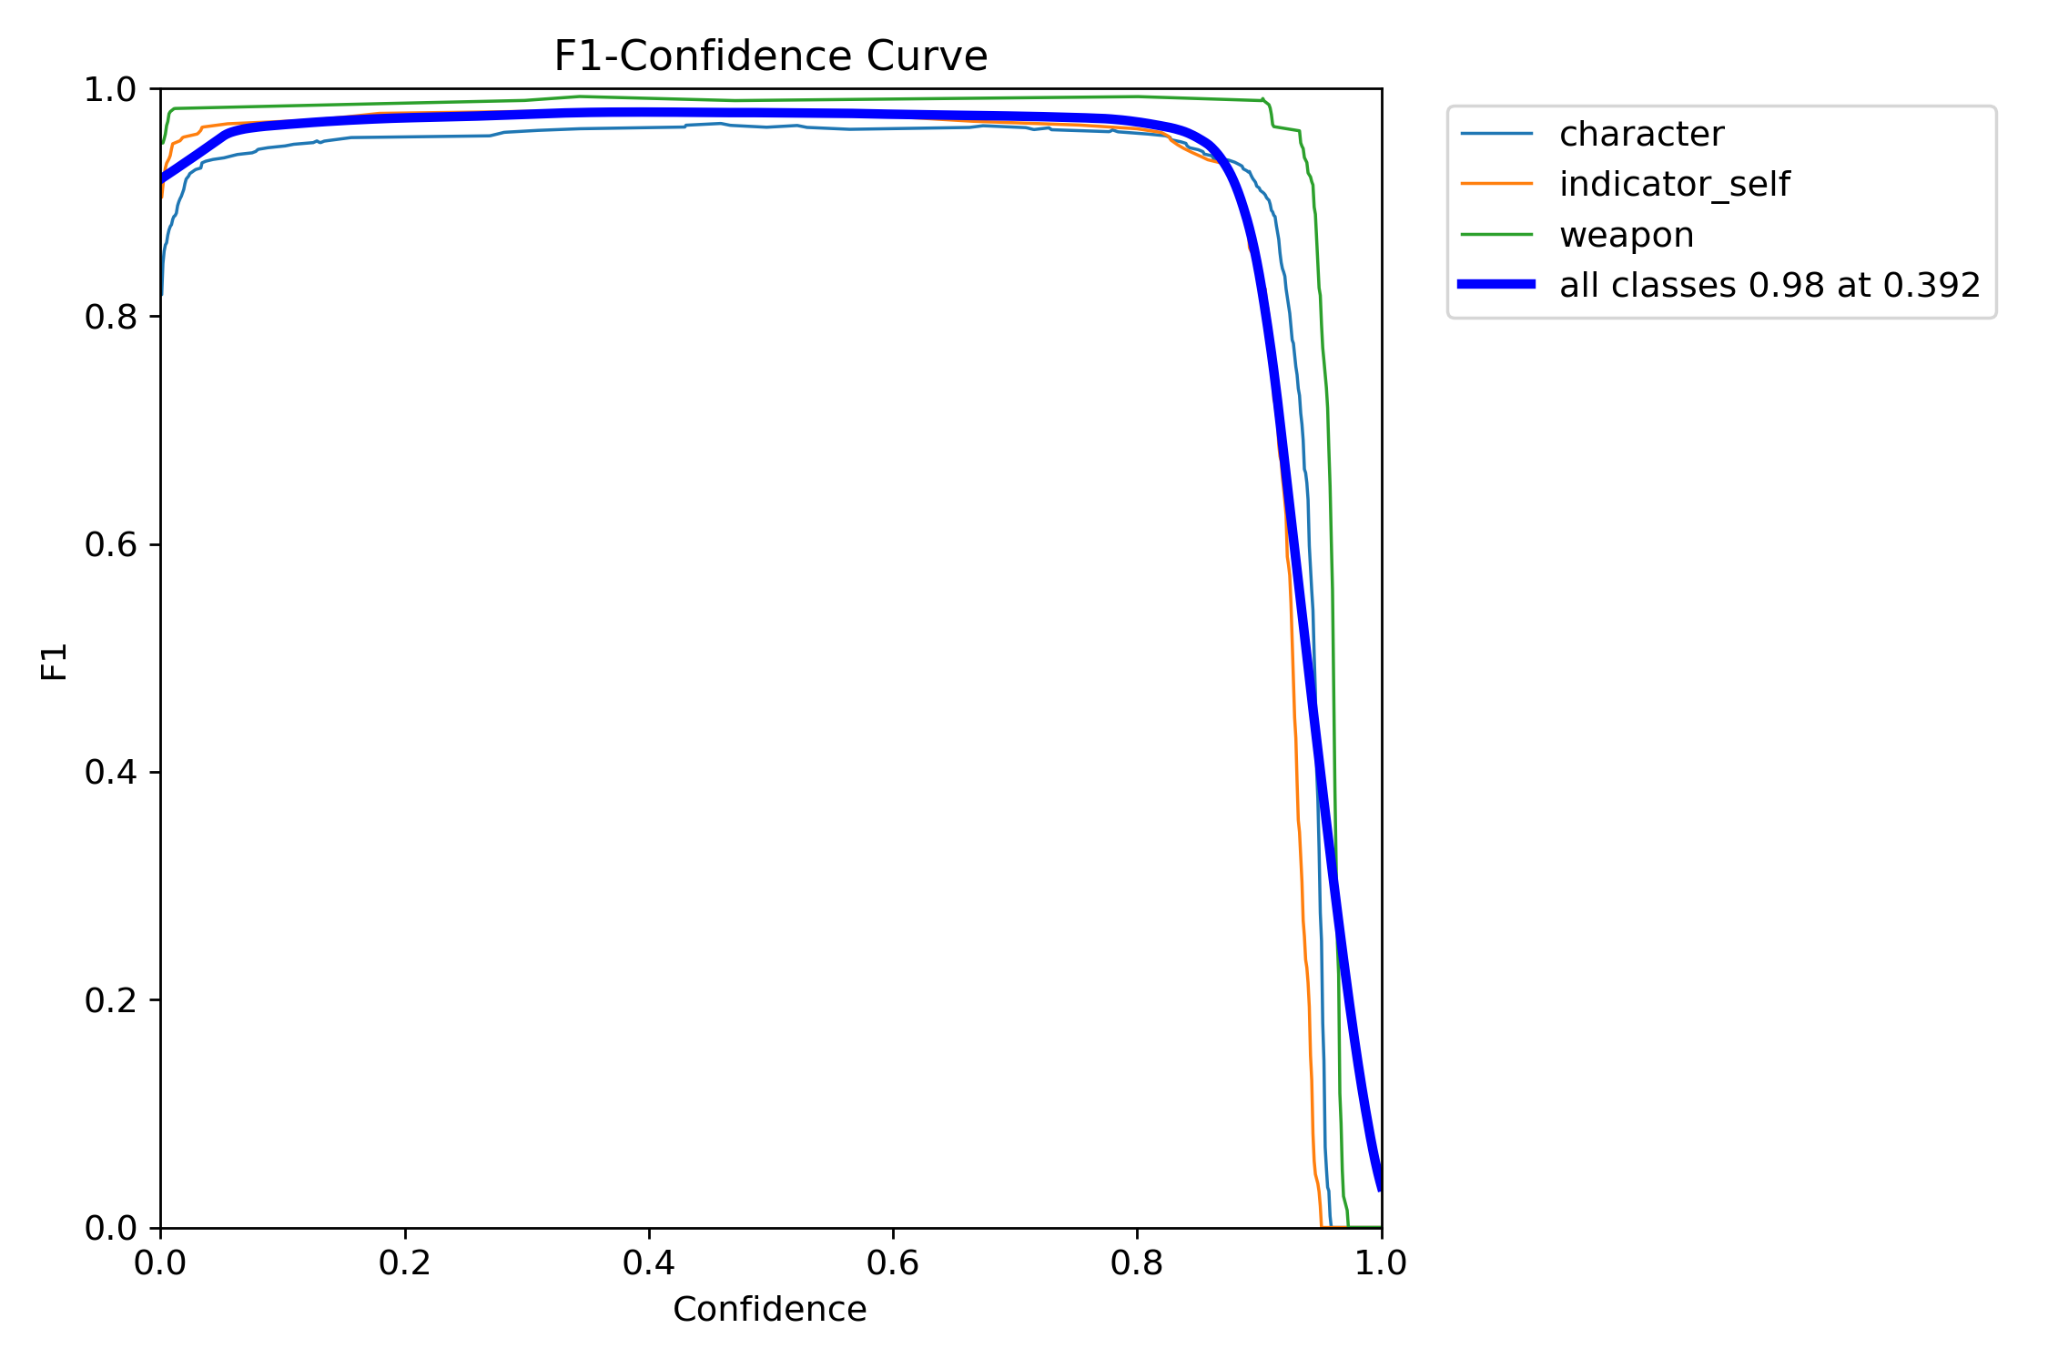
\includegraphics[width=\linewidth]{figures/detector_f1.png}
\caption{F1--confidence curve.}
\end{subfigure}
\caption{Detector validation. Aggregate AP@0.5 is 0.984 and maximum aggregate F1 is 0.98.}
\label{fig:detectorcurves}
\end{figure}

\begin{figure}[t]
\centering
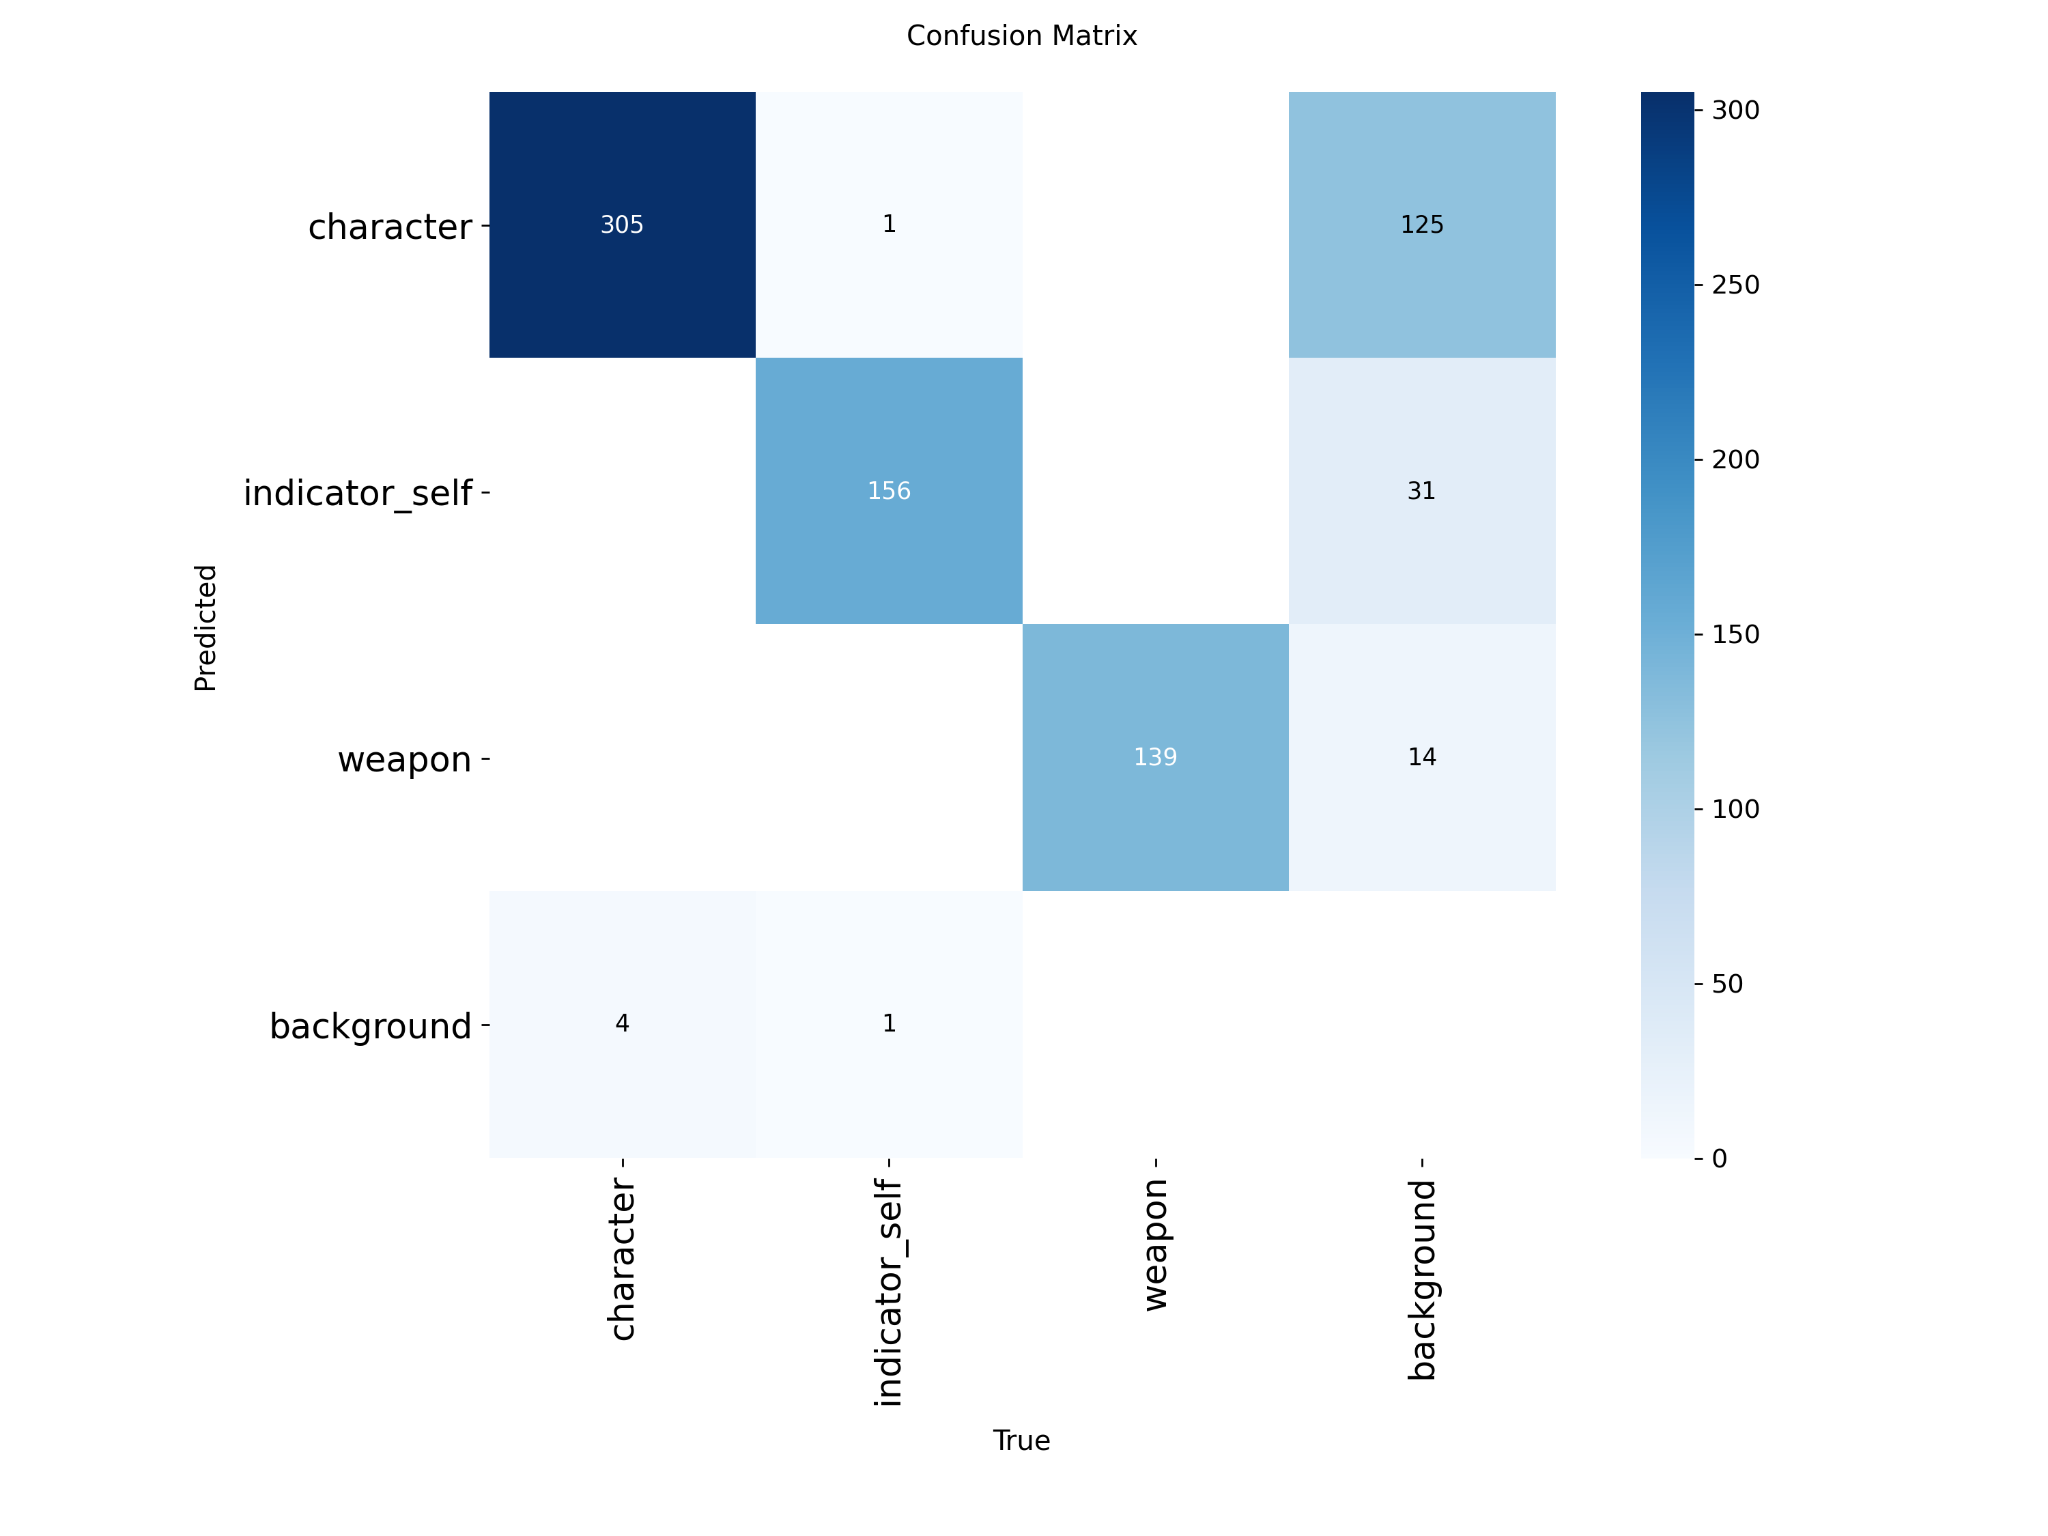
\includegraphics[width=0.78\linewidth]{figures/detector_confusion_matrix.png}
\caption{Detector confusion matrix supplied by the validation run. Background-associated false predictions remain even with high AP, including 125 character, 31 self-indicator, and 14 weapon predictions against background in the displayed summary.}
\label{fig:cm}
\end{figure}

These results establish strong offline perception but do not establish semantic correctness of the RL state. The teacher/missingness failure occurred downstream of a detector that itself performed very well.

\subsection{Real-time loop}
System profiling reports a baseline loop of 36.36 ms (27.51 Hz), improved to 32.62 ms (30.7 Hz). The baseline detector path consumed 33.72 ms, or 92.7\% of loop time, while isolated TensorRT inference was approximately 17 ms. Perception therefore dominates the control budget, and end-to-end latency cannot be inferred from isolated network inference alone.

\section{Results II: Superseded Pilot as a Forensic Case Study}
The initial three-hour sequential campaign produced the skill-score matrix in \Cref{fig:oldretention}. These are real logged measurements but \invalidated{must not be interpreted as estimates of the corrected method}.

\begin{figure}[t]
\centering
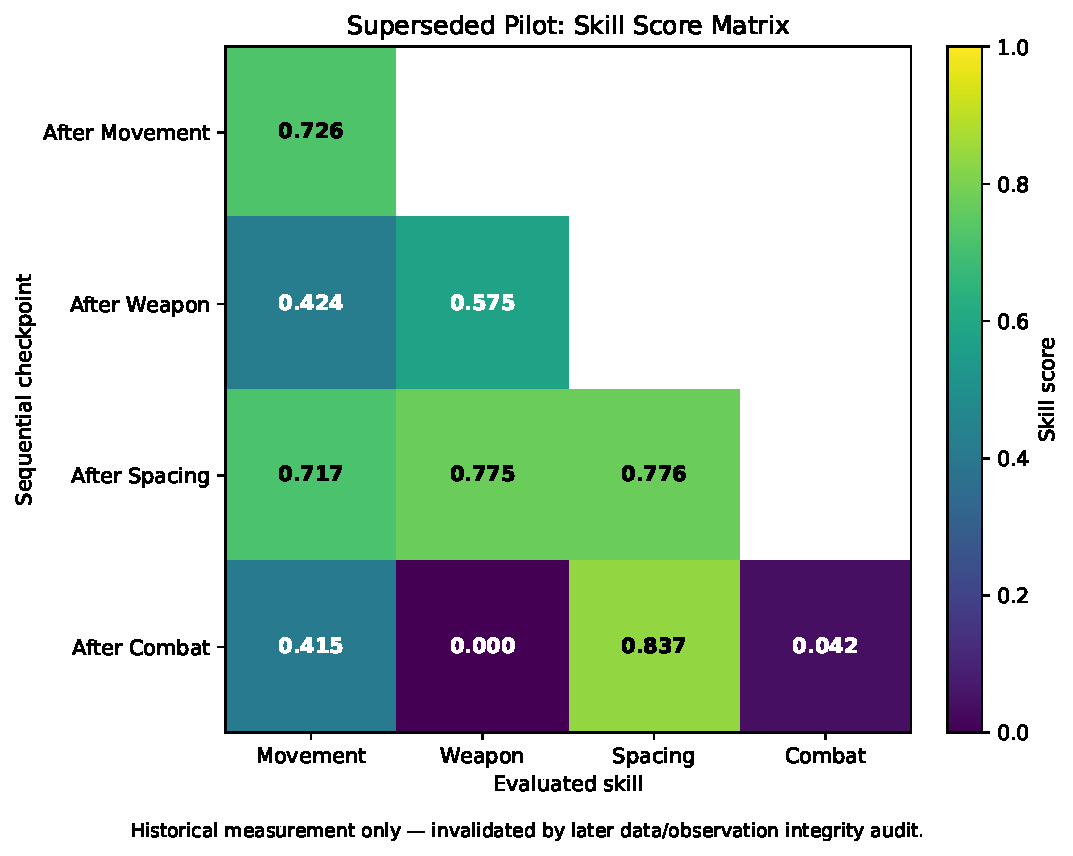
\includegraphics[width=0.74\linewidth]{figures/superseded_retention_matrix.pdf}
\caption{\invalidated{Superseded pilot.} Skill scores after each sequential checkpoint. The apparent total loss of weapon competence after combat was initially consistent with catastrophic forgetting, but later audit showed the weapon teacher/data semantics were invalid.}
\label{fig:oldretention}
\end{figure}

The exact historical matrix is
\begin{equation}
\mathbf S_{\mathrm{pilot}}\approx
\begin{bmatrix}
0.726 & - & - & -\\
0.424 & 0.575 & - & -\\
0.717 & 0.775 & 0.776 & -\\
0.415 & 0.000 & 0.837 & 0.042
\end{bmatrix}.
\end{equation}
After weapon training, movement had retention 0.584 and amnesia 0.416. After spacing, movement and weapon apparently recovered to skill scores 0.717 and 0.775. After combat, movement was 0.415, weapon was 0.000, spacing was 0.837, and combat itself was only 0.0417.

The episode logs also show a strong non-vacuity warning. In the supplied three-hour logs, 26.4\% of spacing episodes were a single step, compared with 1.2\% for movement, 0.6\% for weapon, and 0\% for combat (\Cref{fig:onestep}). This is not identical to the demonstration-archive audit, but independently shows how a goal-dependent phase can generate inflated episode counts without corresponding behavioral complexity.

\begin{figure}[t]
\centering
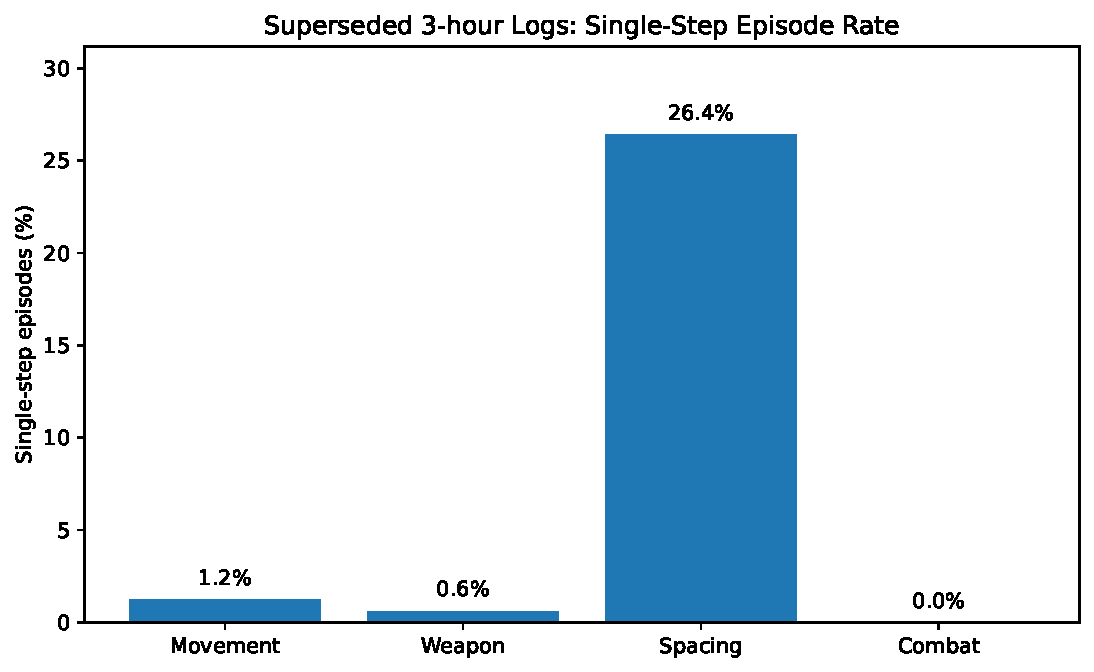
\includegraphics[width=0.72\linewidth]{figures/superseded_single_step_rates.pdf}
\caption{Single-step episode rates in the supplied superseded three-hour episode logs. Spacing is the clearest warning signal at 26.4\%.}
\label{fig:onestep}
\end{figure}

The correct interpretation of this pilot is therefore methodological: \emph{retention gates and cross-skill evaluation made the abnormal behavior visible enough to trigger a deeper data audit}. The pilot does not establish that the final continual-learning method catastrophically forgets weapon acquisition.

\section{Results III: Projected Corrected Outcomes}
This section is intentionally written in final-paper form but uses searchable placeholders. Replace every \texttt{\textbackslash projected\{...\}} value with measured output from the repaired chain.

\subsection{Skill acquisition and retention}
The working hypothesis is that the repaired sequential policy will produce diagonal skill scores approximately
\begin{equation}
S_{M,M}=\projected{0.84},\quad
S_{W,W}=\projected{0.88},\quad
S_{S,S}=\projected{0.85},\quad
S_{C,C}=\projected{0.58}.
\end{equation}
Combat is deliberately projected lower because successful combat depends on longer temporal interaction, opponent response, and attack selection rather than primarily geometric goal satisfaction.

\begin{table}[t]
\centering
\caption{Projected format for the corrected triangular skill-score matrix. Replace every projected value with measured output.}
\label{tab:projectedmatrix}
\begin{tabular}{lrrrr}
\toprule
Checkpoint after & Movement & Weapon & Spacing & Combat\\
\midrule
Movement & \projected{0.84} & -- & -- & --\\
Weapon & \projected{0.81} & \projected{0.88} & -- & --\\
Spacing & \projected{0.82} & \projected{0.85} & \projected{0.85} & --\\
Combat & \projected{0.78} & \projected{0.80} & \projected{0.81} & \projected{0.58}\\
\bottomrule
\end{tabular}
\end{table}

These placeholders imply final retentions
\begin{align}
R_M&=\projected{0.929}, & A_M&=\projected{0.071},\\
R_W&=\projected{0.909}, & A_W&=\projected{0.091},\\
R_S&=\projected{0.953}, & A_S&=\projected{0.047},
\end{align}
and mean final retention
\begin{equation}
\bar R=\projected{0.930}.
\end{equation}

\todofig{\textbf{Corrected retention matrix.} Replace with a heatmap generated from the repaired \texttt{*\_retention\_eval.csv} files. Mark any cell with $R<0.85$ and report the evaluation episode count in the caption.}

\subsection{Learning curves}
For every skill, report return, goal error, goal-success fraction, and the task-specific skill score against cumulative environment interactions. Avoid smoothing that hides instability; provide the raw or lightly smoothed curve and state the window explicitly.

\todofig{\textbf{Corrected learning curves.} Four panels or one shared-axis plot for movement, weapon, spacing, and combat. X-axis: cumulative live-game transitions. Y-axis: normalized skill score; secondary figure may show mean goal error.}

\section{Transfer Efficiency}
Define interactions-to-criterion for skill $i$ at threshold $S^*$ as
\begin{equation}
T_i(S^*)=\min\{t:S_i(t)\ge S^*\}.
\end{equation}
The interaction reduction from transferred initialization is
\begin{equation}
\mathrm{IR}_i=1-\frac{T_i^{\mathrm{transfer}}}{T_i^{\mathrm{scratch}}}.
\end{equation}
A normalized learning-curve area is
\begin{equation}
\mathrm{AUC}=\frac{1}{T}\int_0^T S(t)\,dt,
\end{equation}
and forward transfer can be summarized by
\begin{equation}
FT_i=\frac{\mathrm{AUC}_i^{\mathrm{transfer}}-\mathrm{AUC}_i^{\mathrm{scratch}}}{|\mathrm{AUC}_i^{\mathrm{scratch}}|+\epsilon}.
\end{equation}

\begin{table}[t]
\centering
\caption{Projected transfer-efficiency table.}
\label{tab:transfer}
\begin{tabular}{lrrr}
\toprule
Skill & Scratch interactions & Transfer interactions & Reduction\\
\midrule
Weapon & \projected{14.2k} & \projected{8.7k} & \projected{38.7\%}\\
Spacing & \projected{16.1k} & \projected{10.6k} & \projected{34.2\%}\\
Combat & \projected{28.4k} & \projected{19.3k} & \projected{32.0\%}\\
\midrule
Mean & -- & -- & \projected{35.0\%}\\
\bottomrule
\end{tabular}
\end{table}

Projected AUC-based forward-transfer values are \projected{+0.31} for weapon, \projected{+0.27} for spacing, and \projected{+0.21} for combat.

\todofig{\textbf{Scratch vs transfer.} For each later skill, overlay matched-budget scratch and transferred learning curves. Report threshold $S^*$, interactions-to-criterion, and bootstrap confidence intervals over repeated evaluations.}

\section{Ablation Plan}
The final paper should distinguish representation, transfer, and preservation mechanisms rather than presenting them as one inseparable bundle. The minimum useful ablation set is:
\begin{enumerate}[leftmargin=1.4em]
  \item skill-specific PPO from scratch;
  \item UVFA with simple concatenation;
  \item UVFA + residual FiLM;
  \item + sequential behavioral transfer;
  \item full method without replay/KL preservation;
  \item full method without gradient surgery;
  \item full method.
\end{enumerate}

\begin{table}[t]
\centering
\caption{Projected result shape for the ablation study. These values are not measurements.}
\label{tab:ablation}
\begin{tabular}{lrrr}
\toprule
Method & Mean skill score & Final retention & Combat\\
\midrule
Skill PPO scratch & \projected{0.56} & -- & \projected{0.39}\\
UVFA concat & \projected{0.64} & \projected{0.79} & \projected{0.45}\\
UVFA + FiLM & \projected{0.69} & \projected{0.82} & \projected{0.49}\\
+ BC transfer & \projected{0.73} & \projected{0.84} & \projected{0.54}\\
$-$ replay/KL & \projected{0.74} & \projected{0.72} & \projected{0.57}\\
$-$ PCGrad & \projected{0.75} & \projected{0.82} & \projected{0.57}\\
Full & \projected{0.79} & \projected{0.93} & \projected{0.58}\\
\bottomrule
\end{tabular}
\end{table}

The expected qualitative signature is more important than the placeholder magnitudes: FiLM should primarily improve cross-goal representation; behavioral transfer should primarily improve early sample efficiency; replay/anchoring should primarily improve retention; and gradient surgery should matter most when current and preservation gradients directly conflict.

\section{Transfer to Goal-Independent Match Play}
Skill pretraining is not the final deployment objective. The final policy removes explicit goals:
\begin{equation}
\pi_\psi(a\mid s),
\end{equation}
with parameters initialized from the skill-pretrained representation. The frozen benchmark specifies 30 deterministic matches, one stock to win, and promotion criteria of at least 18 wins, nonnegative mean damage trade, and self-destruct rate at most 0.2.

\begin{table}[t]
\centering
\caption{Projected final-match result. Replace with measured benchmark output and a matched-budget scratch baseline.}
\label{tab:match}
\begin{tabular}{lr}
\toprule
Metric & Projected value\\
\midrule
Matches & \projected{30}\\
Wins & \projected{20}\\
Losses & \projected{10}\\
Win rate & \projected{66.7\%}\\
Wilson 95\% CI & \projected{48.8--80.8\%}\\
Mean damage trade & \projected{+9.4}\\
Self-destruct rate & \projected{0.10}\\
\bottomrule
\end{tabular}
\end{table}

A positive match result is evidence of useful transfer only if compared with a scratch policy using a matched real-interaction budget.

\section{Discussion}
\subsection{Goal conditioning as behavioral representation learning}
The goal interface is useful even if the deployment policy is ultimately goal-independent. During pretraining, the shared representation must support object-directed movement, opponent-relative positioning, pickup, and attack behavior under the same parameters. This makes the GCRL phase a structured representation-learning curriculum rather than merely a permanent high-level controller.

\subsection{Why the integrity failures matter scientifically}
The project provides a concrete counterexample to a common assumption:
\begin{equation}
\text{high offline model accuracy}\;\not\Rightarrow\;\text{valid RL experiment}.
\end{equation}
The detector reached 0.984 mAP@0.5 while a missing-object sentinel still corrupted teacher semantics. Dataset validators returned PASS while successful episodes could be vacuous. Numerical transition arrays were finite and correctly shaped while mutable storage could violate temporal identity. These are not optimization failures; they are failures of the experimental object being optimized.

A more complete validity condition is therefore
\begin{equation}
\boxed{
\begin{aligned}
\text{valid RL evidence}={}&\text{accurate measurement}+\text{correct semantics}\\
&+\text{temporal integrity}+\text{causal task validity}.
\end{aligned}}
\end{equation}

\subsection{Real-time interaction changes the value of sample efficiency}
At approximately 30 control decisions per second, $10^5$ environment steps correspond to roughly 55.6 minutes of uninterrupted interaction even before menus, resets, evaluation, or optimizer downtime are counted. A genuine 35\% reduction in interactions-to-criterion would therefore be practically meaningful, not merely a plotting improvement.

\section{Limitations}
The current study is intentionally narrow. The principal configuration uses one controlled legend (Wu Shang), one Easy Mordex opponent, one map, and one opponent policy. Generalization across legends, weapons, maps, and stronger or adaptive opponents remains untested. Real-time training cost limits the number of complete independent seeds; repeated evaluation episodes reduce checkpoint-evaluation uncertainty but do not substitute for multi-seed optimization. The goal vocabulary and reward structure encode substantial prior knowledge. Recovery and all-skill consolidation were deferred in the initial pilot. Some historical world-replay data are invalidated by the observation-aliasing bug, and all pre-repair weapon conclusions must be treated cautiously. Finally, every \projected{placeholder} in this manuscript must be replaced before scientific submission.

\section{Conclusion}
We presented a vision-only reinforcement-learning system for skill acquisition and transfer in a live commercial fighting game. The architecture combines goal-conditioned UVFA learning, residual FiLM modulation, behavioral initialization, sequential transfer, PPO, replay-based preservation, policy anchoring, and gradient-conflict mitigation. The perception system is already strong, reaching 0.984 mAP@0.5 and maximum aggregate F1 0.98, while the control loop operates near 30 Hz.

The most important finding to date is methodological. An initial sequential campaign appeared to show severe forgetting, including a measured weapon score of zero after combat training. That interpretation was invalidated after audit exposed missing-value semantics, mutable observation aliasing, and vacuous successes. The result is not an excuse to hide the failed run; it is evidence that retention gates and transition-integrity checks are necessary in real-world RL systems.

The repaired experiment will test two explicit hypotheses: sequential GCRL transfer reduces interactions-to-criterion by approximately \projected{35\%}, and replay/anchoring/gradient conflict handling preserve approximately \projected{93\%} of earlier competency after the combat phase. The manuscript is structured so those hypotheses can be replaced directly by the corrected measurements without rewriting the methodological argument.

\appendix
\section{Numerical Replacement Ledger}
Search the source for \texttt{\textbackslash projected\{} or the rendered token \textbf{[P:...]} before submission. At minimum, replace:
\begin{itemize}[leftmargin=1.4em]
  \item corrected evaluation episode count;
  \item four diagonal skill scores and every off-diagonal retention evaluation;
  \item final retention/amnesia and mean retention;
  \item scratch-vs-transfer interaction counts, AUCs, and confidence intervals;
  \item all ablation values;
  \item final match benchmark, Wilson interval, damage trade, and self-destruct rate;
  \item corrected transition totals and exact training wall-clock if they differ from the working protocol.
\end{itemize}

\section{Required Final Figures}
\begin{enumerate}[leftmargin=1.4em]
  \item representative gameplay frame with perception overlays;
  \item system architecture (already included as a TikZ overview; replace with a more detailed version if desired);
  \item detector PR/F1 plots (included);
  \item corrected learning curves;
  \item scratch-vs-transfer curves;
  \item corrected triangular retention heatmap;
  \item superseded historical matrix (included and explicitly labelled);
  \item ablation summary;
  \item final match benchmark comparison;
  \item qualitative frame sequences for movement, weapon acquisition, spacing, and combat;
  \item optional integrity-failure schematic showing sentinel misuse, aliasing, and vacuous success.
\end{enumerate}

\section{Reproducibility Checklist}
For each final result archive, store:
\begin{itemize}[leftmargin=1.4em]
  \item clean git SHA and worktree/content hash;
  \item frozen config and manifest hashes;
  \item demo/replay data hashes;
  \item policy checkpoint hash;
  \item random seed;
  \item exact game setup, resolution, detector engine, and auxiliary classifier checkpoint;
  \item training and evaluation wall-clock intervals;
  \item integrity-test outputs;
  \item raw episode, step, and retention-evaluation CSV files.
\end{itemize}

\begin{thebibliography}{9}

\bibitem[Schaul et~al.(2015)Schaul, Horgan, Gregor, and Silver]{schaul2015uvfa}
T. Schaul, D. Horgan, K. Gregor, and D. Silver.
\newblock Universal Value Function Approximators.
\newblock In \emph{Proceedings of the 32nd International Conference on Machine Learning}, 2015.

\bibitem[Perez et~al.(2018)Perez, Strub, de~Vries, Dumoulin, and Courville]{perez2018film}
E. Perez, F. Strub, H. de Vries, V. Dumoulin, and A. Courville.
\newblock FiLM: Visual Reasoning with a General Conditioning Layer.
\newblock In \emph{AAAI Conference on Artificial Intelligence}, 2018.

\bibitem[Schulman et~al.(2017)Schulman, Wolski, Dhariwal, Radford, and Klimov]{schulman2017ppo}
J. Schulman, F. Wolski, P. Dhariwal, A. Radford, and O. Klimov.
\newblock Proximal Policy Optimization Algorithms.
\newblock arXiv:1707.06347, 2017.

\bibitem[Andrychowicz et~al.(2017)Andrychowicz et~al.]{andrychowicz2017her}
M. Andrychowicz et al.
\newblock Hindsight Experience Replay.
\newblock In \emph{Advances in Neural Information Processing Systems}, 2017.

\bibitem[Yu et~al.(2020)Yu et~al.]{yu2020pcgrad}
T. Yu et al.
\newblock Gradient Surgery for Multi-Task Learning.
\newblock In \emph{Advances in Neural Information Processing Systems}, 2020.

\bibitem[Kirkpatrick et~al.(2017)Kirkpatrick et~al.]{kirkpatrick2017ewc}
J. Kirkpatrick et al.
\newblock Overcoming Catastrophic Forgetting in Neural Networks.
\newblock \emph{Proceedings of the National Academy of Sciences}, 114(13):3521--3526, 2017.

\bibitem[Mnih et~al.(2015)Mnih et~al.]{mnih2015dqn}
V. Mnih et al.
\newblock Human-Level Control through Deep Reinforcement Learning.
\newblock \emph{Nature}, 518:529--533, 2015.

\bibitem[Vinyals et~al.(2019)Vinyals et~al.]{vinyals2019alphastar}
O. Vinyals et al.
\newblock Grandmaster Level in StarCraft II Using Multi-Agent Reinforcement Learning.
\newblock \emph{Nature}, 575:350--354, 2019.

\end{thebibliography}

\end{document}
